\documentclass[11pt, a4paper]{article}
\usepackage[utf8x]{inputenc}
\usepackage[sort]{natbib}
\setcounter{tocdepth}{4}
\setcounter{secnumdepth}{4} 

\usepackage[spanish]{babel}
\usepackage{enumitem}
\usepackage{graphicx}
\usepackage{float}
\usepackage[linktoc=all]{hyperref}

\usepackage{etoolbox}

\usepackage{amsmath}
\usepackage{amssymb}
\usepackage{array}
\usepackage{gensymb}

\usepackage{fancyhdr}
\usepackage[table]{xcolor}
\usepackage{color}
\usepackage{colortbl}
\definecolor{lightgray}{gray}{0.9}
\setlength{\columnsep}{0.5cm}


%------------------- Dimensiones -------------------
\usepackage{geometry}
 \geometry{a4paper,total={170mm,257mm},left=15mm,right=15mm,top=20mm,}
%----------------------------------------------------

%------------------- Encabezado y Pie de pág -------------------
\pagestyle{fancy}
\fancyhf{}
\lhead{Técnicas Digitales IV}
\rhead{TP1}
\rfoot{Página \thepage}
%----------------------------------------------------


%----------------------------- Documento -----------------------------------------------
\begin{document}
\begin{titlepage}
 \centering
	
\includegraphics[scale=0.80]{Imagenes/LOGO.jpg} \par
 	\vspace{1cm}
 	{\scshape\LARGE Universidad Tecnológica Nacional \par}
 	{\scshape\large Facultad Regional de Córdoba \par}
 	\vspace{1cm}
	{\bfseries \Large Trabajo Práctico De Laboratorio $N^{\circ} 1$\par}
 	\vspace{1.5cm}

	\begin{tabular}{ll}
		Navarro, Facundo		&	63809 	
	\end{tabular}
	
	\vspace{1cm}
	Curso: 6r4 \\
	Grupo $N^{\circ} 5$
 	\vfill
	{\bfseries \Large Técnicas Digitales IV\par}

	\vspace{1.5cm}
	Docentes: \par
	Ing. Cayuela, Pablo \par
	Ing. Olmedo, Sergio \par

 	\vfill
	{\large \today\par}
\end{titlepage}
	
	
\tableofcontents
\clearpage

\section{Introducción}
	El siguiente informe documenta los procedimientos realizados para el diseño digital de un controlador de un motor mediante la lectura de un encoder, se utilizar parte de las prácticas adquiridas en los prácticos de entrenamiento y se profundiza en los conocimientos sobre encoders o codificadores rotativos. 

\section{Marco Teórico}
	\subsection{Encoder}
	Un ``encoder rotatorio", también llamado codificador del eje o generador de pulsos, es un dispositivo electromecánico capaz de convertir la posición angular de un eje a un código digital. Estos dispositivos suelen ser añadidos a motores de corriente continua para convertir el movimiento mecánico en pulsos digitales que pueden ser interpretado por un sistema electrónico de control. 

	Encuentran aplicación dentro de los campos de la robótica, lentes fotográficas, aplicaciones industriales que requieran medición angular, etc.

	Los motores DC tienen un comportamiento complejo en cuanto a control de posición y de la velocidad, el cual no es lineal y depende mucho de la carga que soporten, es por este motivo que surge la necesidad de la aplicación de un encoder que permita conocer y asegurar la correcta posición del eje.

	Según su diseño y funcionalidad existen distintos tipos de encoders. Los tipos más comunes se pueden clasificar en absolutos y relativos.

	\subsubsection{Encoder Absoluto}
	Un encoder absoluto es un dispositivo que mide la posición absoluta angular. Esta diseñado para proporcionar un código digital de acuerdo a la posición angular de la flecha, como se ve en la imagen \textcolor{blue}{\textbf{\ref{fig:encoder_absoluto}}}, una vuelta esta dividida en un número especifico de divisiones o marcas y cada una de ellas se les asigna físicamente un código digital único, es decir, que tiene un código único para cada posición. 

\begin{figure}[h]
	\centering
	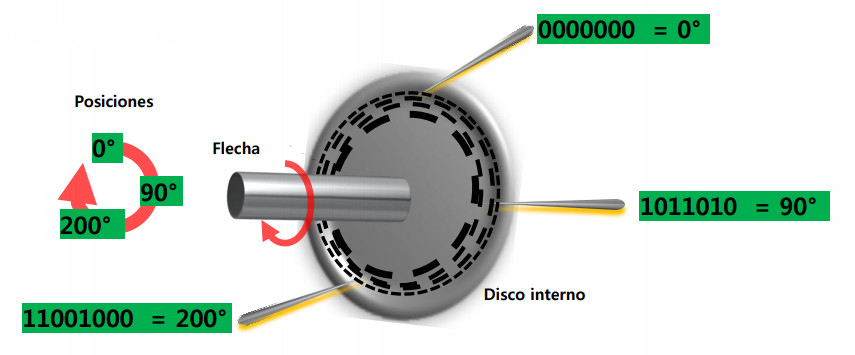
\includegraphics[width=0.8\textwidth]{Imagenes/encoder_absoluto.jpg}
	\caption{Estructura interna de un encoder absoluto.}
	\label{fig:encoder_absoluto}
\end{figure} 

\subsubsection{Encoder Incremental}
 El tipo común de encoder incremental consiste de un disco solidario al eje del motor que contiene un patrón de marcas o ranuras que son codificados por un interruptor óptico generando pulsos eléctricos cada vez que el patrón del disco interrumpe y luego permite el paso de luz hacia el interruptor óptico a medida que el disco gira. 

 Este tipo de encoders determina la posición de rotación de acuerdo a un número específico de pulsos por vuelta (PPV), mediante el conteo de esos pulsos a medida que el encoder gira, es entonces que la PPV es un factor de resolución y es el aspecto más importante a la hora de seleccionar un encoder incremental.  La resolución de un encoder típico es del orden de 1000 pulsos por revolución.

 Desde un encoder incremental no se puede determinar la posición angular absoluta del eje. Para poder determinar la posición relativa a un punto de referencia (cero), el encoder debe incluir una señal adicional que genera un pulso por revolución, denominada ``Indice" (Z).

\begin{figure}[h]
	\centering
	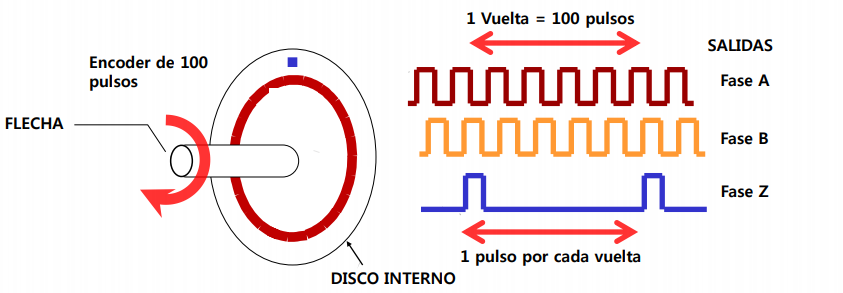
\includegraphics[width=0.8\textwidth]{Imagenes/encoder_incremental.jpg}
	\caption{Estructura interna de un encoder incremental.}
	\label{fig:encoder_incremental}
\end{figure} 

\subsubsection{Encoder en cuadratura}
Corresponde a un tipo de encoder incremental que utiliza dos sensores ópticos posicionados con un desplazamiento de 1/4 de ranura el uno del otro, generando dos señales de pulsos digitales desfasadas en 90 grados o en ``cuadratura". Estas señales se llaman comúnmente $A$ y $B$, mediante ellas es posible suministrar los datos de posición, velocidad y dirección de rotación del eje.

Usualmente, si la señal A adelanta a B (la señal A toma un valor lógico de ``1" antes que B) se establece por convenio que el eje esta rotando en sentido horario, mientras que si B adelanta a A, el sentido es anti horario, como se ve en la figura \textcolor{blue}{\textbf{\ref{fig:encoder_cuadratura}}}.
\begin{figure}[h]
	\centering
	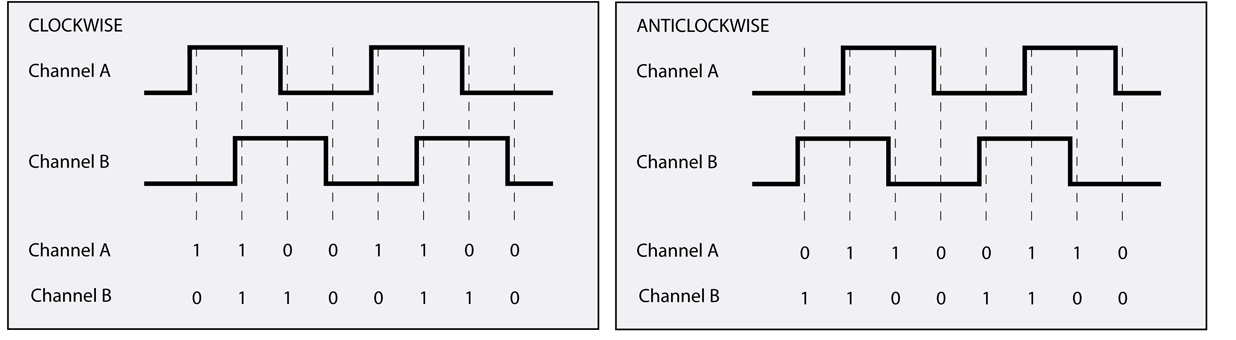
\includegraphics[width=0.8\textwidth]{Imagenes/encoder_cuadratura.jpg}
	\caption{Sentido de giro del encoder en cuadratura}
	\label{fig:encoder_cuadratura}
\end{figure} 

\clearpage
\section{Control de lazo cerrado en posición de un motor C.C.}
\subsection{Consigna}
	Realizar la descripción de un decodificador de encoder incremental visualizando en un display los pulsos en n\_contador\_up\_down.

	Con la cuenta se debe controlar una señal PWM. Esta señal, el ciclo de trabajo debe variar entre $5\%$ y $95\%$. La frecuencia debe ser de 400 Hz.

	El ciclo de trabajo al 50\% del PWM, debe suceder cuando la comparación de la cuenta del contador\_up\_down es igual a la entrada de referencia.

	La entrada de referencia, nos dice en que lugar se quiere posicionar el motor, dentro de una revolución indicada por la cuenta desde 0 a 1999 pulsos de encoder.

	La entrada debe ser de 11bit, como tambien el contador\_up\_down.

	La señal PWM debe ser maxima para una diferencia $\pm 100$ entre la cuenta de los pulsos (contador\_up\_down) y la de referencia.


\subsection{Modificaciones}
	Se modificó levemente la consigna para sacar provecho del hardware disponible, se utiliza un encoder de 1440 PPV, por lo cual es necesario incrementar el contador y la cantidad de bits necesaria para representar esta nueva magnitud.

\subsection{Desarrollo}

	\subsubsection{Estructura del proyecto}
	El proyecto fue desarrollado en el SW Vivado 2019.2.1, ya que se utilizo la plataforma de entrenamiento de Digilent Basys3.

	\begin{figure}[H]
		\centering
		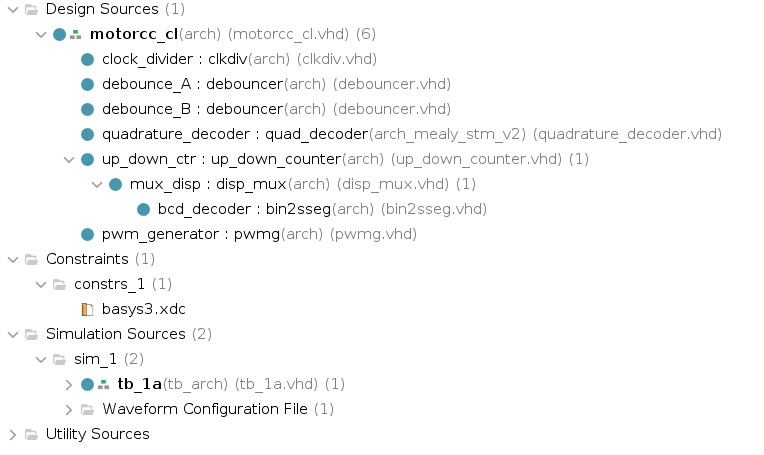
\includegraphics[width=0.7\textwidth]{Imagenes/estructura.png}
		\caption{Árbol del proyecto}
		\label{fig:proyecto_vivado}
	\end{figure} 

	\subsubsection{Debouncer}
	Siempre existe la posibilidad de ruido externo que se puede introducir dentro de la señal, en este caso se plantea un filtro digital a través de un registro, el cual podría ser parametrizado en caso que se requiera un tiempo mayor para estabilizar la señal.

	\begin{figure}[H]
		\centering
		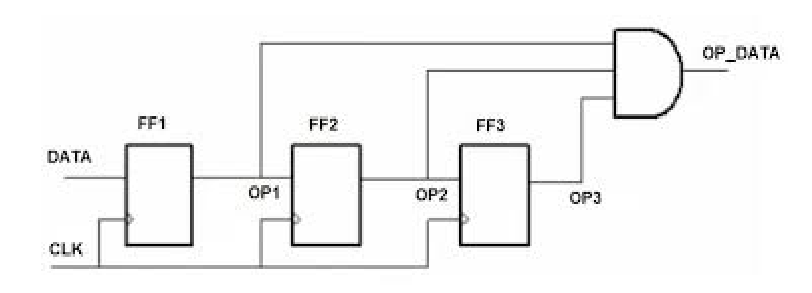
\includegraphics[width=0.5\textwidth]{Imagenes/debouncer.png}
		\caption{Estructura de filtro digital.}
		\label{fig:debouncer}
	\end{figure} 

	El filtro se utiliza sobre las señales que provienen del encoder, A y B como se aprecia en la imagen \textcolor{blue}{\textbf{\ref{fig:A_B}}}.

	\begin{figure}[H]
		\centering
		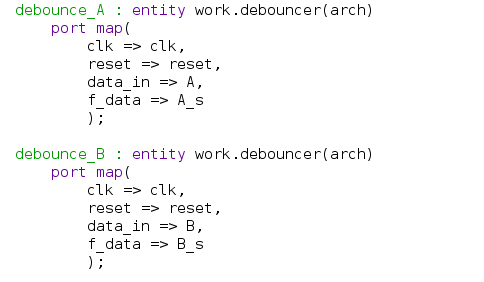
\includegraphics[width=0.5\textwidth]{Imagenes/A_B.png}
		\caption{Señales filtradas A y B.}
		\label{fig:A_B}
	\end{figure} 


	\subsubsection{Divisor de frecuencia y multiplexado de displays}
			A partir de la frecuencia de la placa $f_1$ en 100 MHz, se pretende utilizarla para realizar el multiplexado de los 4 displays necesarios para visualizar la cuenta hasta 5759, como el ojo no es capaz de percibir el encendido y apagado a alta velocidad, fenómeno conocido como persistencia de la visión, engañando al espectador en creer que el los displays se encuentran encendido en simultáneo.
		\begin{equation}
			f_{mux} = \frac{f_{in}}{2^n} = \frac{100Mhz}{2^{17}} \approx 800 Hz
		\end{equation}

			Con la frecuencia de 100 Mhz, es necesario un registro de 19 bits de longitud, con los 2 MSB se multiplexa la salida de los display a una velocidad aproximada de 800 Hz.
		\begin{figure}[H]
			\centering
			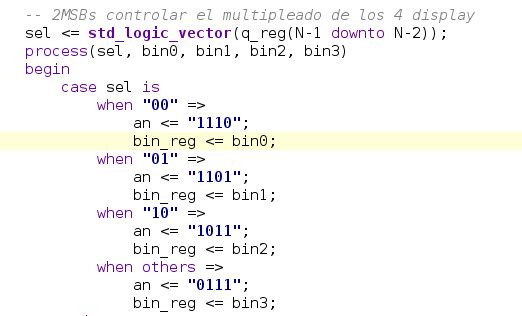
\includegraphics[width=0.5\textwidth]{Imagenes/mux.png}
			\caption{Multiplexado de displays de 7 segmentos.}
			\label{fig:mux}
		\end{figure} 
		
		
	\subsubsection{Decodificador de cuadratura}
			El decodificador del encoder en cuadratura se plantea como una máquina de estado que detecta el sentido de acuerdo si la señal A se adelanta a señal B o su inversa. Por cada transición del nivel bajo hacia alto o bajo se produce un pulso. Como se dijo previamente, una características principal de este tipo de encoder es su resolución, el encoder utilizado tiene una resolución de 1440 ppv, la cual se multiplica por 4, correspondiendo a un ciclo entero entre las señales en cuadratura A y B, otorgando una mayor resolución de 5760 ppv, haciendo necesario un contador de módulo 5760.
		\begin{figure}[H]
			\centering
			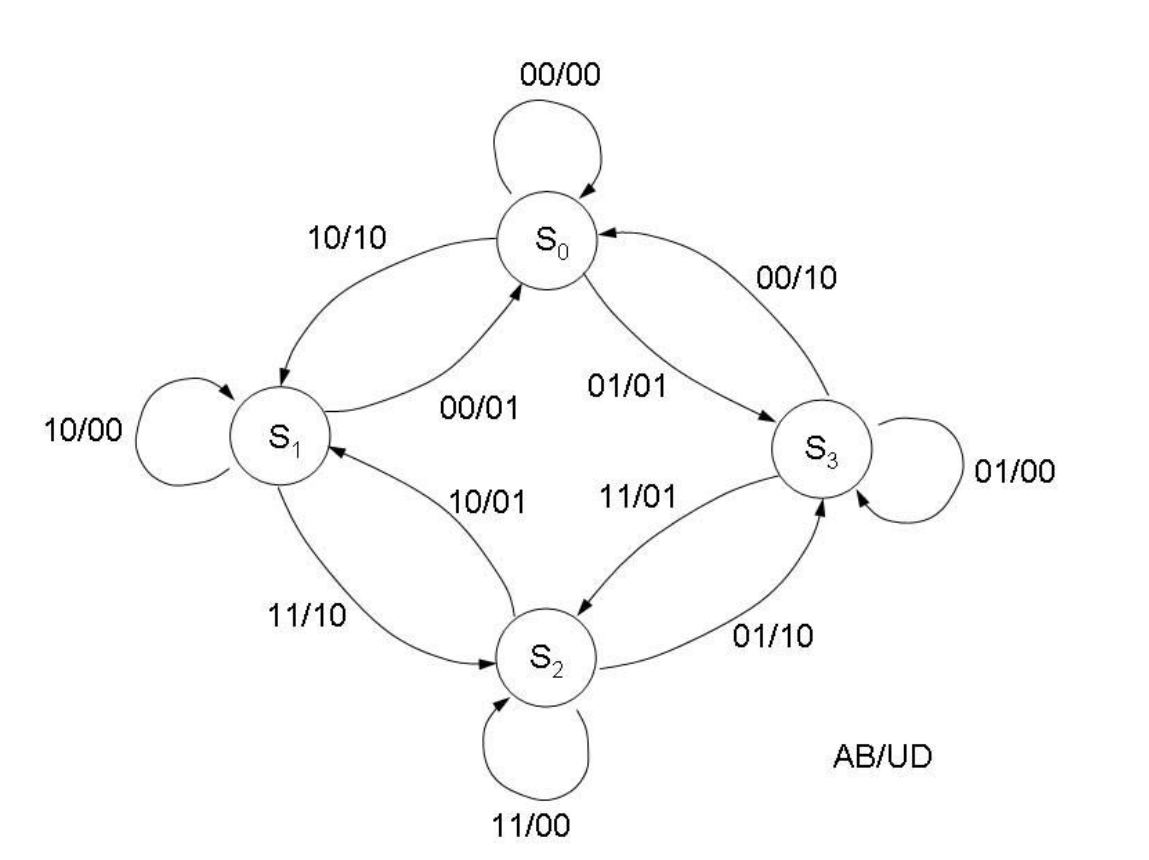
\includegraphics[width=0.6\textwidth]{Imagenes/mealy.jpg}
			\caption{Máquina de Mealy}
			\label{fig:mealy}
		\end{figure} 
		
		Los resultados de la máquina de Mealy se observan en la imagen \textcolor{blue}{\textbf{\ref{fig:mealy_tb}}}, aclarando que se probaron 3 arquitecturas distintas en la descripción, dos mealy y un combinacional puro.

		\begin{figure}[H]
			\centering
			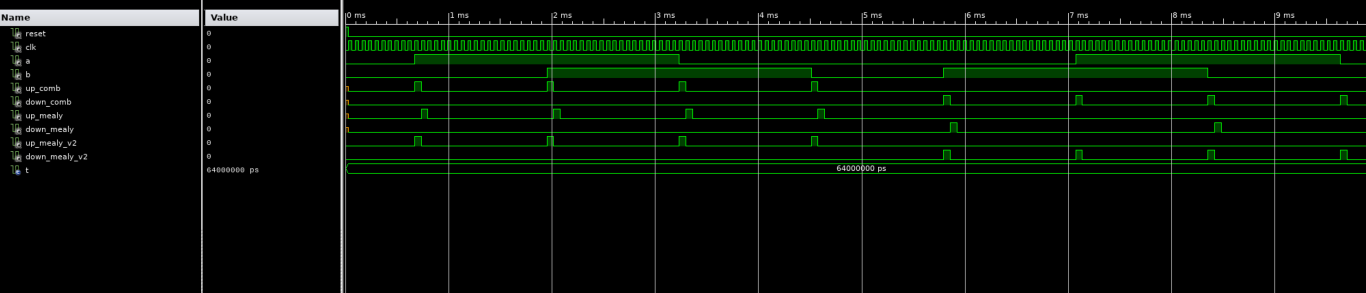
\includegraphics[width=\textwidth]{Imagenes/tb_mealy.png}
			\caption{Simulación de detector de cuadratura.}
			\label{fig:mealy_tb}
		\end{figure} 
\clearpage

	\subsubsection{Contador 0 - 5759}
			El encoder incremental usado se ve en la imagen \textcolor{blue}{\textbf{\ref{fig:encoder_real}}} 

		\begin{figure}[H]
			\centering
			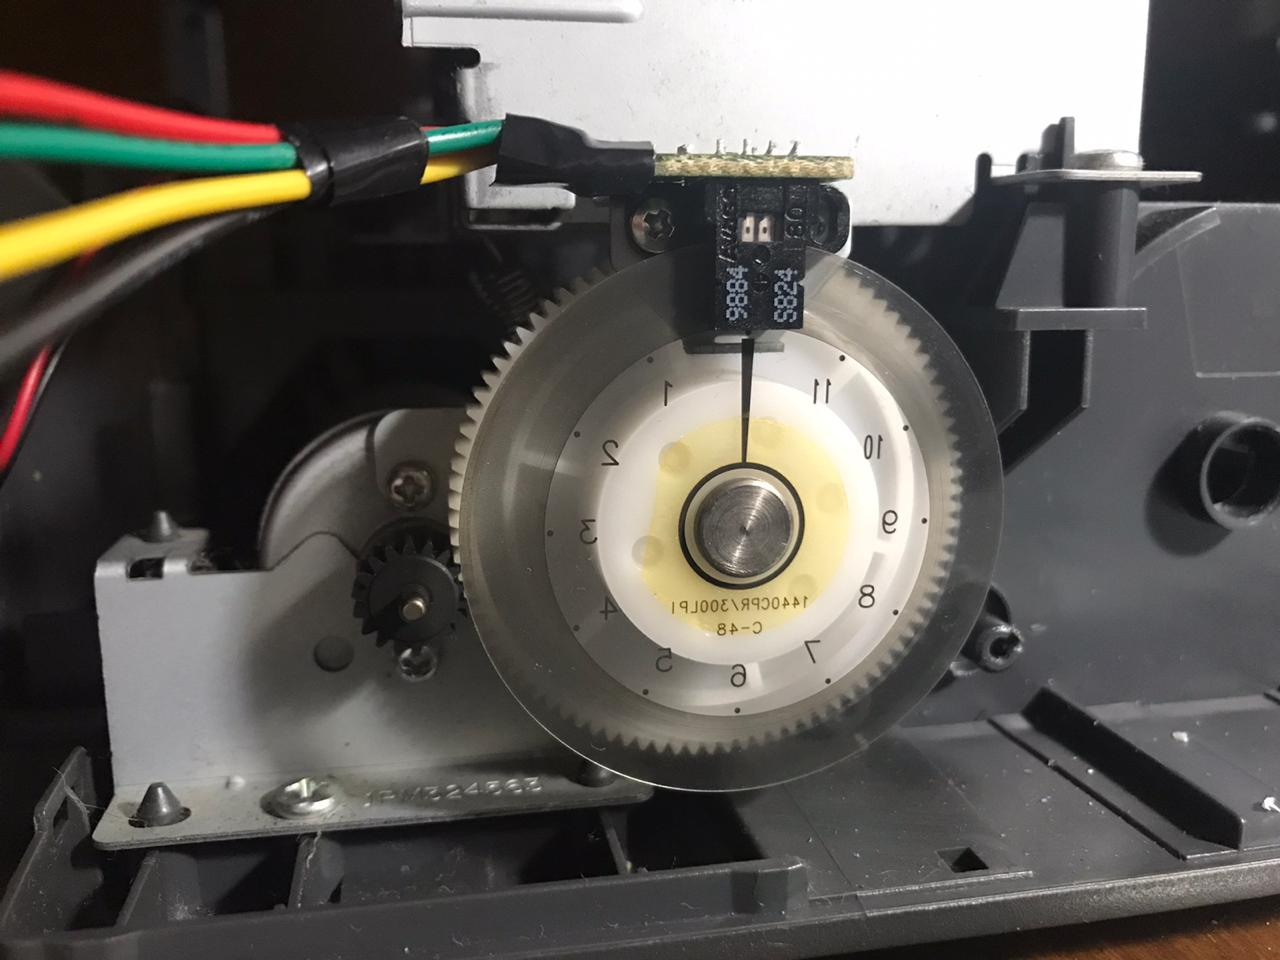
\includegraphics[width=0.5\textwidth]{Imagenes/encoder_real.jpeg}
			\caption{Encoder de 1440 ppv.}
			\label{fig:encoder_real}
		\end{figure} 

			Para el contador de módulo 5760, se usan los pulsos que se generan en el detector de cuadratura, de acuerdo si la señal es \textit{up} o \textit{down}, el valor de contador asciende o desciende respectivamente. Como se ve en la figura \textcolor{blue}{\textbf{\ref{fig:M}}}, si en algún momento se acierta uno de los pulsos y además concuerda con el valor parametrizable \textit{M} o \textit{M\_n}, el valor de registro se setea a 0.

		\begin{figure}[H]
			\centering
			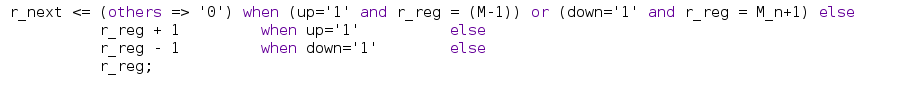
\includegraphics[width=\textwidth]{Imagenes/mod5760.png}
			\caption{Contador módulo 5760.}
			\label{fig:M}
		\end{figure} 

		Para los displays en un principio se orientó la solución utilizando un conversor binario a BCD, el cual consiste en un registro de desplazamiento con una adición de un entero de valor 6 de acuerdo si se cumplen ciertas condiciones, el mismo se implementó y se vio que tenia el resultado correcto, sin embargo se trataba de una estructura que consumía muchos recursos y necesita de muchos pulsos de clock para convertir una entrada serie, a una salida paralela de 12 bit para los 4 displays, caso por el cual se implementa un contador similar al planteado en los ejercicios de entrenamiento (10).

		\begin{figure}[H]
			\centering
			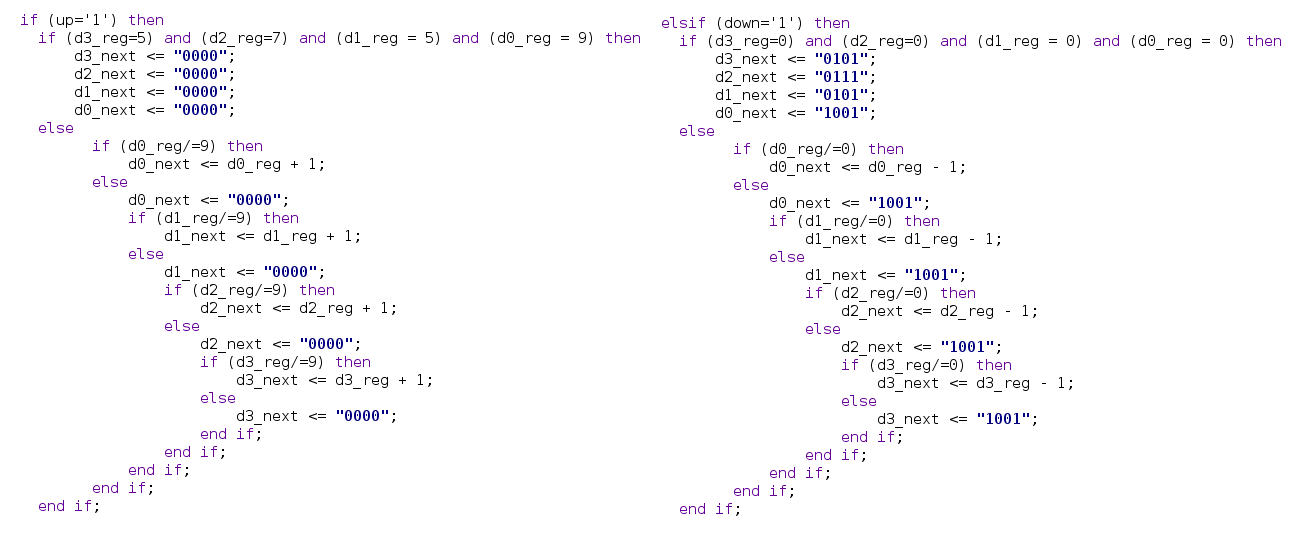
\includegraphics[width=0.8\textwidth]{Imagenes/updown.png}
			\caption{Descripción de contador para displays 7 segmentos.}
			\label{fig:updown}
		\end{figure} 
		
		En la imagen \textcolor{blue}{\textbf{\ref{fig:updown}}} se puede apreciar que se utilizan 4 registros de 4 bits (dn\_reg) para cada uno de los displays, en el caso de que se acierte un pulso \textit{up}, se incrementa los registros de los displays, con la condición que si el valor previo era 9, el próximo valor posible es 0. Para el caso inverso, con el pulso \textit{down} la lógica es similar, pero en este caso los registros se decrementan, con la excepción que si el valor es 0 el siguiente valor sera 9.
		Por ultimo se debe notar la condición que si el contador llega a un valor equivalente 5759 y se acierta un pulso up, los registros se reinician, caso contrario si se encuentra en 0 y se acierta un pulso down, el los registros se establecen a 5759.
	
	\subsubsection{PWM}
			Para el control del motor se genera dos señales de PWM en contra fase, las cuales son utilizadas para controlar tanto la velocidad como el sentido de giro del motor. Estas señales son llevadas a una llave H, formada por un integrado L9110S, el comportamiento de la llave con las señales es la siguiente:
			\begin{itemize}
				\item{Duty $=$ 50\%} : Motor parado en torque.
				\item{Duty $>$ 50\%}: Motor gira en sentido horario.
				\item{Duty $<$ 50\%}: Motor gira en sentido anti horario.
			\end{itemize}

		\paragraph{Frecuencia del PWM}
				Como requisito se pedía una frecuencia de 400 Hz. Para ello se debe tener en cuenta la resolución del PWM, como así también la frecuencia del clock. Se elige una resolución de 7 bit para satisfacer la condición de un mínimo de 5\% y un máximo de 95 \%. 

				\begin{equation}
					f_{out} = \frac{f_{clk}}{2^{(n+1)}} = \frac{100\;Mhz}{2^18} \approx 381 Hz
				\end{equation}
	
				Restando los 7 bit de resolución del PWM se debe elegir el divisor de frecuencia correspondiente a Q(10), como se muestra en la imagen \textcolor{blue}{\textbf{\ref{fig:clk_div}}}.

		\begin{figure}[H]
			\centering
			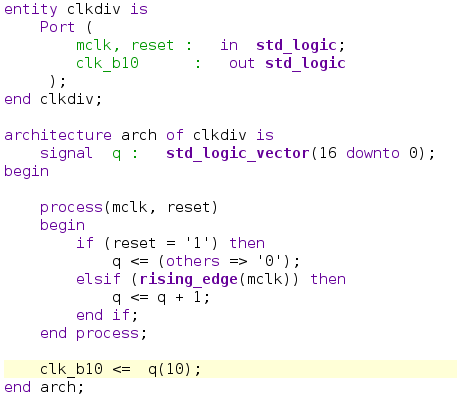
\includegraphics[width=0.5\textwidth]{Imagenes/clk_div.png}
			\caption{Divisor de frecuencia}
			\label{fig:clk_div}
		\end{figure} 

		De esta manera se tiene el clock del PWM, falta ajustar el periodo necesario para llegar a 400 Hz
			\begin{equation}
				T = \frac{T_{buscada}}{T_{clk\_div}} * 2^n = \frac{2,5 \; ms}{2,62 \; ms} * 128 \approx 122 
			\end{equation}

		\begin{figure}[H]
			\centering
			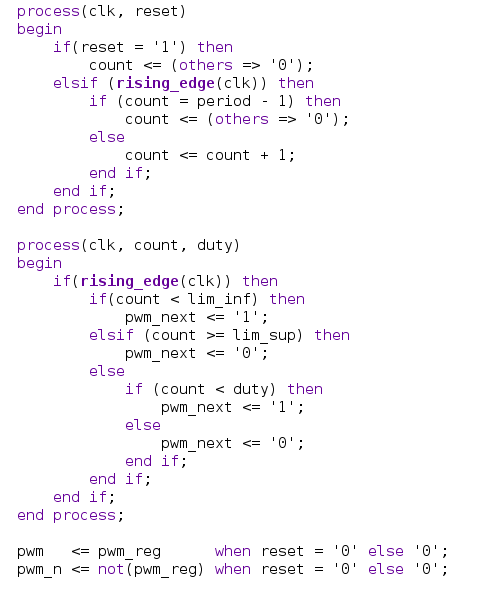
\includegraphics[width=0.5\textwidth]{Imagenes/pwm_400.png}
			\caption{Descripción de PWM}
			\label{fig:pwm_400}
		\end{figure} 

		Finalmente, se pide que si los pasos entre la posición actual del motor y la de referencia difieren en $\pm 100$, la velocidad es máxima, esto se consigue con la siguiente descripción.

		\begin{figure}[H]
			\centering
			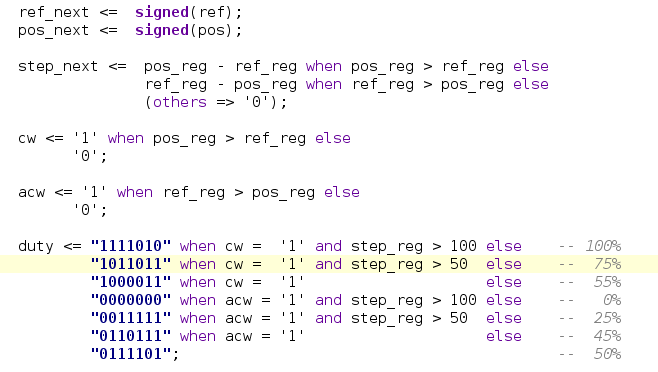
\includegraphics[width=0.5\textwidth]{Imagenes/func_pwm.png}
			\caption{Seleccion de sentido de giro y duty cycle.}
			\label{fig:func_pwm}
		\end{figure} 

		El funcionamiento del código en  \textcolor{blue}{\textbf{\ref{fig:func_pwm}}} es el siguiente, \textit{pos} es derivado del módulo contador y \textit{ref} de los switchs y es variable con estas. Dependiendo cual sea mayor a la otra determinara el sentido de giro, ya sea clockwise(cw) o anticlockwise(acw). Por ultimo se busca la magnitud de separación entre ambas posiciones, si es mayor de 100 se elegirá un pwm mas cercano a la máxima velocidad respetando el sentido de giro, caso que la posición actual sea igual a la referencia, tanto cw y acw valen '0' y el duty queda al 50\% (torque).

		\subsubsection{Simulaciones}
		\begin{figure}[H]
			\centering
			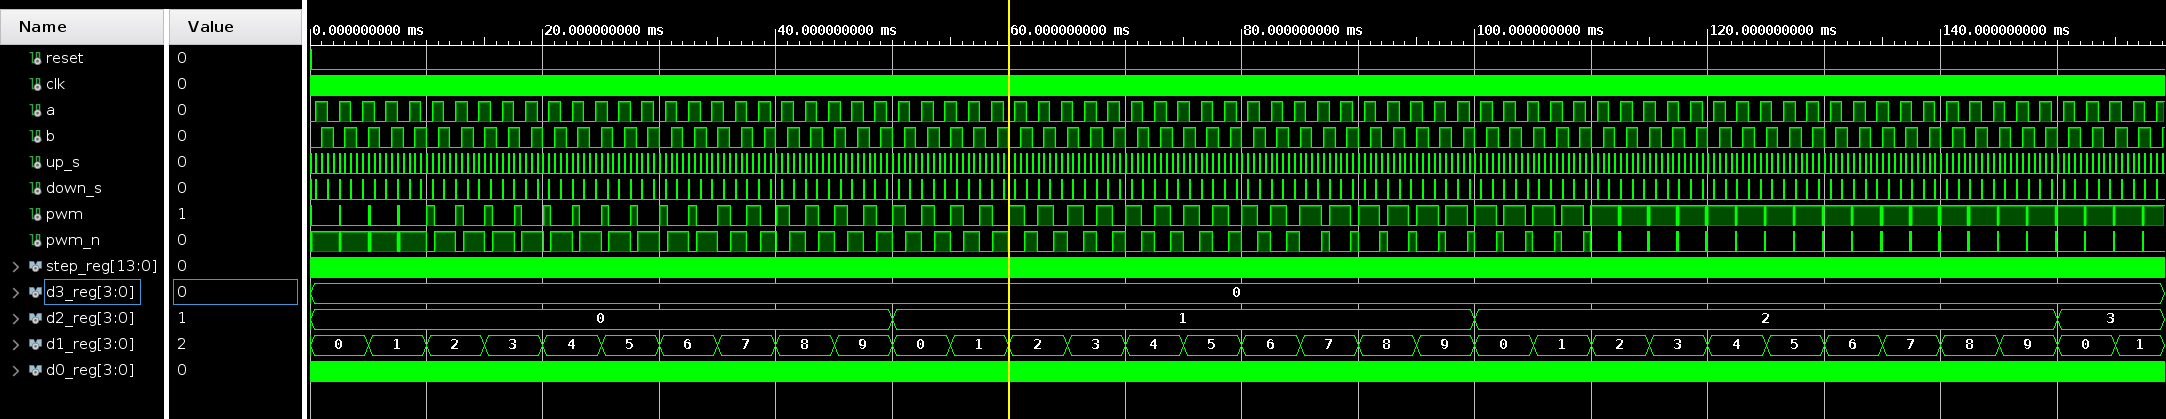
\includegraphics[width=\textwidth]{Imagenes/sim_impl_120.png}
			\caption{Simulación behavioral, con referencia puesta en 120.}
			\label{fig:sim_behav_pwm}
		\end{figure} 

		\begin{figure}[H]
			\centering
			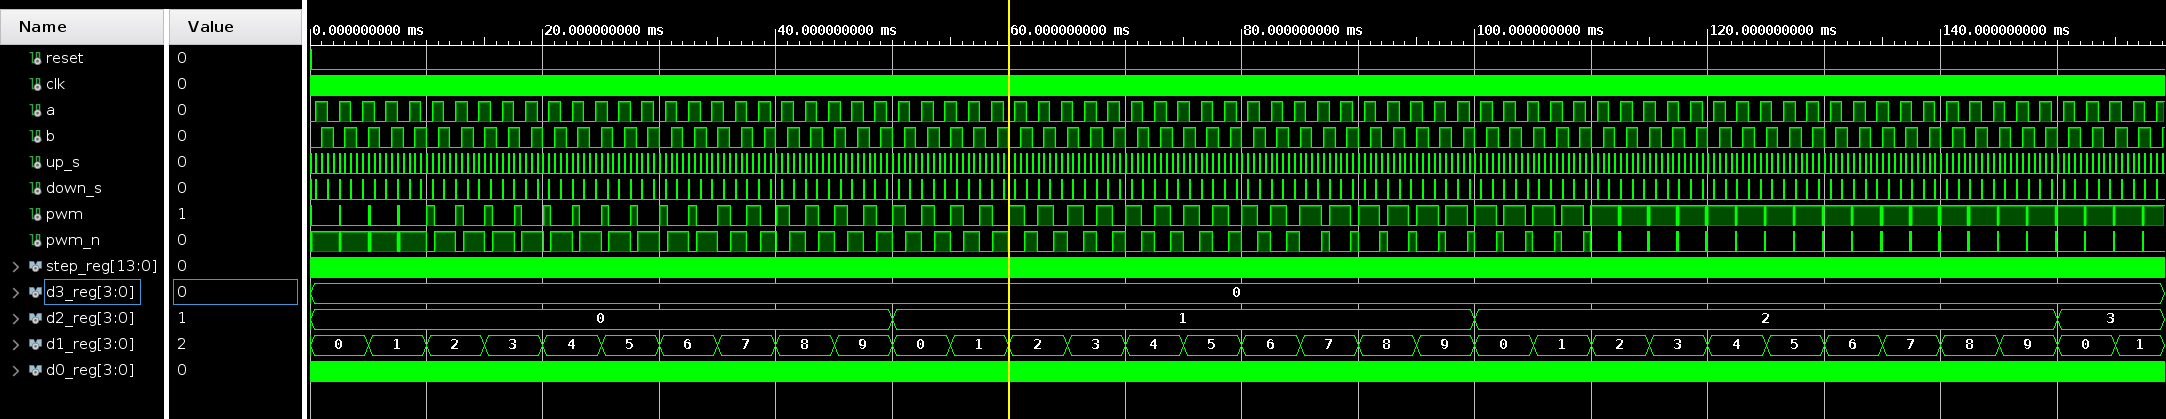
\includegraphics[width=\textwidth]{Imagenes/sim_impl_120.png}
			\caption{Simulación postfit, con referencia puesta en 120.}
			\label{fig:sim_impl_pwm}
		\end{figure} 
		
		\begin{figure}[H]
			\centering
			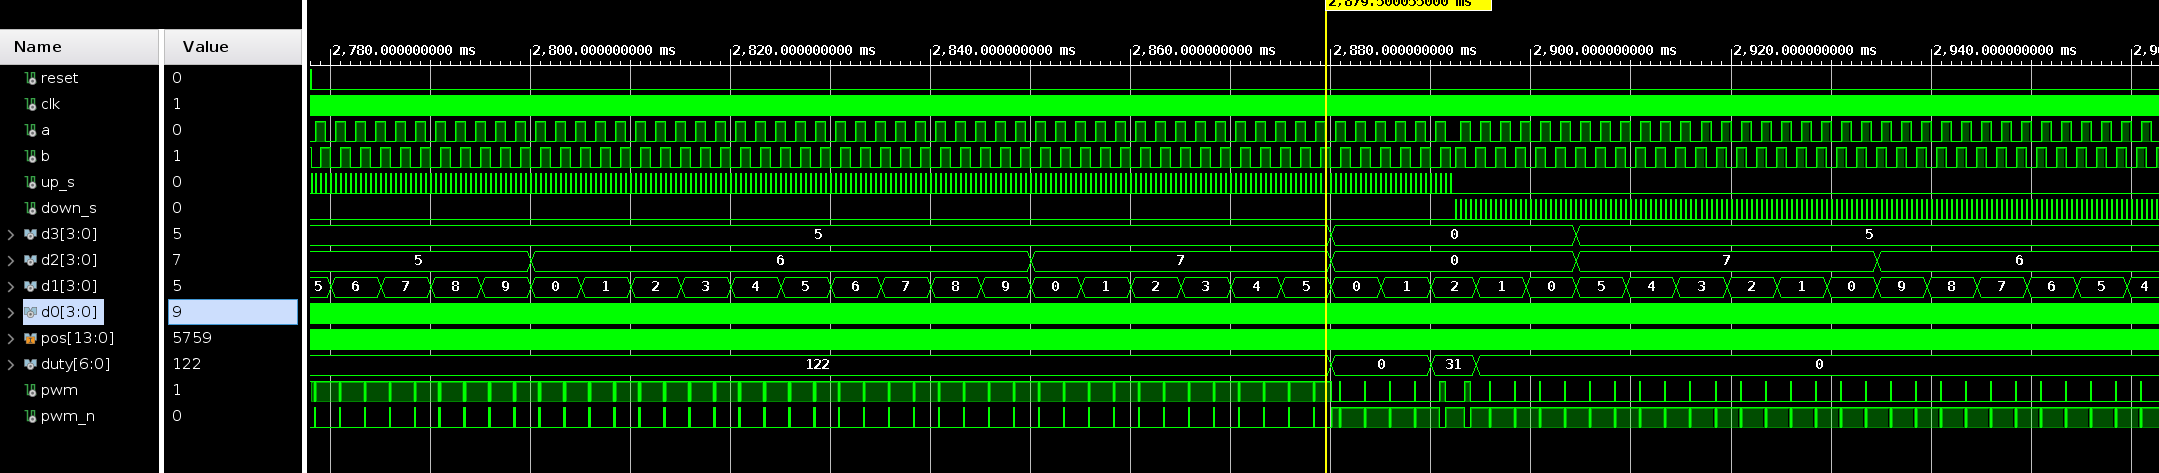
\includegraphics[width=\textwidth]{Imagenes/sim_up.png}
			\caption{Reinicio contador ascendente modulo 5760}
			\label{fig:cont_up}
		\end{figure} 
		
		\begin{figure}[H]
			\centering
			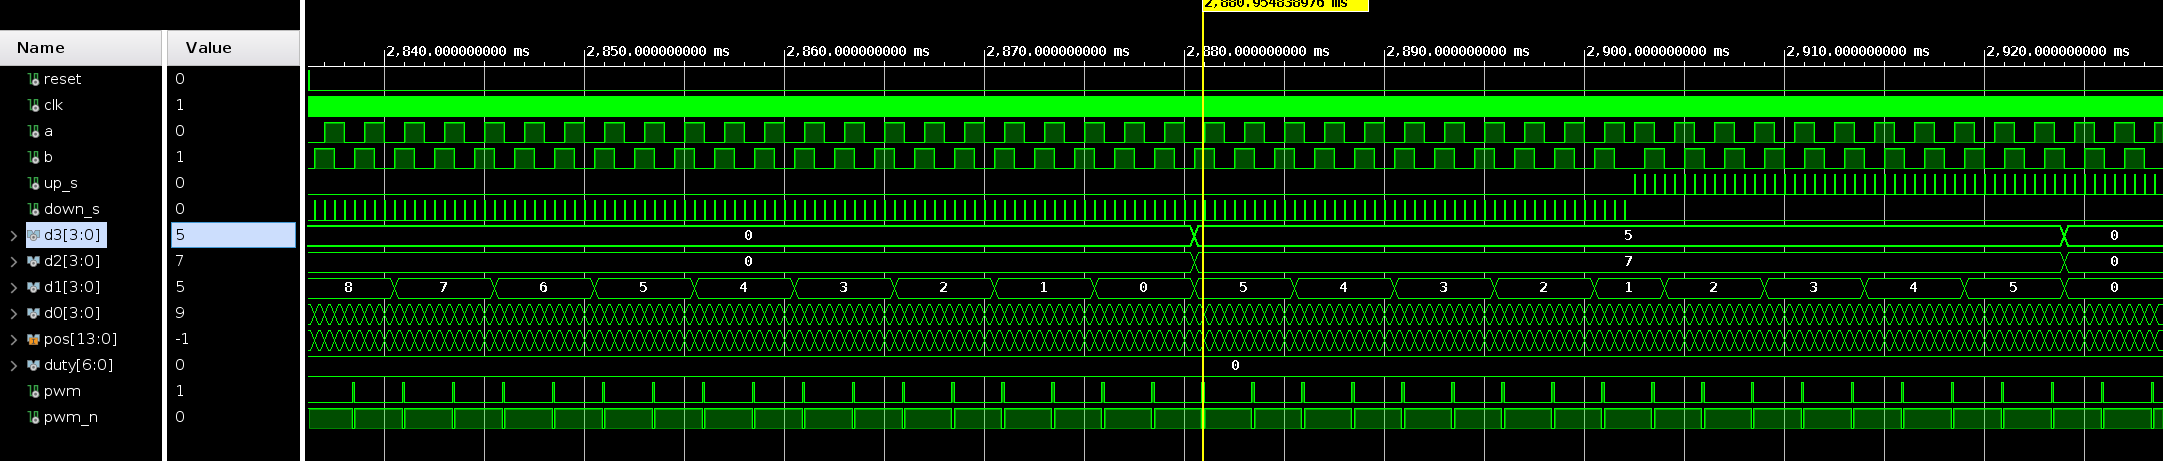
\includegraphics[width=\textwidth]{Imagenes/sim_down.png}
			\caption{Reinicio contador descendente modulo 5760}
			\label{fig:cont_down}
		\end{figure} 

		\subsubsection{Multimedia}
		Se adjunta un dos links de unos vídeos demostrativos: 
		\begin{itemize}
			\item Presentación: \url{https://youtu.be/4qJg4IgcLNk}
			\item Demo: \url{https://youtu.be/wE91018Mobk}
		\end{itemize}
	\section{Control de lazo de velocidad de un motor C.C.}
	\section{Control de motor paso a paso de velocidad a lazo abierto con rampa de aceleración y desale ración parametrizable}
\end{document}
